\section{Why do people watch creative livestreams?}
%t-shape motivations, deep on adobe, then broad
%For every person who livestreams, there are many more people watching. Who are they, and what are their motivations? What benefits and challenges do they experience? 
% xxx: rewording this to shorten a bit, how is this?
Every livestream needs an audience. To understand the motivations and challenges of viewers, we conducted three surveys over 1.5 years with 165 people: two with \textit{Adobe Live} viewers; one with viewers of any creative livestreams on the Web. All three surveys were voluntary. We found that creative livestream viewers watch streams primarily for \textit{learning} and \textit{inspiration}; community engagement and entertainment were also popular reasons for watching streams. Compared with prior work on livestream viewers in other domains, inspiration is a much more prominent theme in these survey responses.
%In particular, the unique combination of learning with entertainment and engagement that livestreams offer makes them an appealing choice over other types of learning-focused content.

\subsection{Survey methodology}
The first survey with \textit{Adobe Live} viewers (\textit{S1}) was posted periodically in the chat and overlaid on the stream for four months (August - December 2017). It asked about viewers' experience with creative software, the reasons they watch creative livestreams, what other creative livestreams they watch besides \textit{Adobe Live}, and how \textit{Adobe Live} streams could be improved. 98 people completed this survey.

A year later, \textit{Adobe Live} had changed considerably: more frequent streams, more audience interaction, and wider and more regular marketing. In January 2019, we conducted \textit{S2} to gain additional insights about viewer motivations and challenges, focusing especially on the live chat experience. The survey was sent directly to previous winners of Adobe's \textit{Daily Creative Challenges} who also showed up regularly in past chat logs of Adobe streams. 41 people completed this survey.

Finally, to zoom out and capture a broader range of creative livestream viewers, we conducted a third survey (\textit{S3}) with viewers of creative livestreams on \textit{any}  platform. The survey was disseminated with a snowball method, via the researchers' personal social media accounts. Participants were required to have viewed creative livestreams before, which were defined as ``activities such as visual art (drawing, painting, etc.), crafts, music performance, cooking, DIY projects, programming, etc.'' This survey asked viewers about the streams they watch, motivations for watching them, examples of things they learned from them, what else they do while watching, and on which platforms they watch. 26 people completed this survey.

\begin{table}[b]
\centering
\resizebox{1\columnwidth}{!}{
\begin{tabular}{lcccc}
          & \textbf{\begin{tabular}[c]{@{}c@{}}Survey 1\\ $n=98$\end{tabular}} & \textbf{\begin{tabular}[c]{@{}c@{}}Survey 2\\ $n=41$\end{tabular}} & \textbf{\begin{tabular}[c]{@{}c@{}}Survey 3\\ $n=26$\end{tabular}} & \textbf{\begin{tabular}[c]{@{}c@{}}Total\\ $n=165$\end{tabular}} \\
YouTube   & 40                                                                 & 17                                                                 & 17                                                                 & 74                                                               \\
Twitch    & 9                                                                  & 4                                                                  & 17                                                                 & 30                                                               \\
Facebook  & 5                                                                  & 4                                                                  & 4                                                                  & 13                                                               \\
Periscope & 1                                                                  & 1                                                                  & 2                                                                  & 4                                                                \\
Instagram & -                                                                  & -                                                                  & 6                                                                  & 6                                                                \\
Phlearn   & 2                                                                  & -                                                                  & -                                                                  & 2                                                               
\end{tabular}
}
\caption{All platforms listed more than once in at least one survey by respondents when asked where they watch creative livestreams.}~\label{table:platforms}
\vspace{-0.15in}
\end{table}

\subsection{What do people watch, and where?}
The most popular platform overall was YouTube (74), with Twitch second (30) (\autoref{table:platforms}). This is likely skewed by the fact that \textit{Adobe Live} is on YouTube. \textit{S3} had a smaller sample size but found YouTube and Twitch to be equally popular.

\textit{S3} respondents listed content genres they frequently watch live. Categories that came up more than once were programming (11/26), cooking (6/26), digital art (\emph{i.e.}, digital painting, photo editing) (5/26), music (4/26), physical artwork (i.e. drawing, painting) (3/26), 3D modeling (2/26), and DIY (2/26).

\subsection{Viewers watch for learning and inspiration}
Viewers responded similarly about motivations in all three surveys. Despite the differences in sample sizes and populations, this suggests that \textit{Adobe Live} viewers' responses may often align with viewers more broadly. Across all three surveys, learning was the most common reason people chose for watching creative livestreams (\autoref{fig:livestream_survey_responses}). While learning has also been found to be an important goal for viewers in other domains such as gaming, the primary goal most often cited in prior work is entertainment \cite{Lu2019, Wohn2018, Lu2018a, Hilvert-Bruce2018, Faas2018, Cheung2011}.
%In culture-sharing livestreams people learn creative skills or techniques \cite{Lu2019}. 
This difference may be due to the prevalence of Teaching livestreams in creative communities.

\begin{figure}[b!]
\centering
  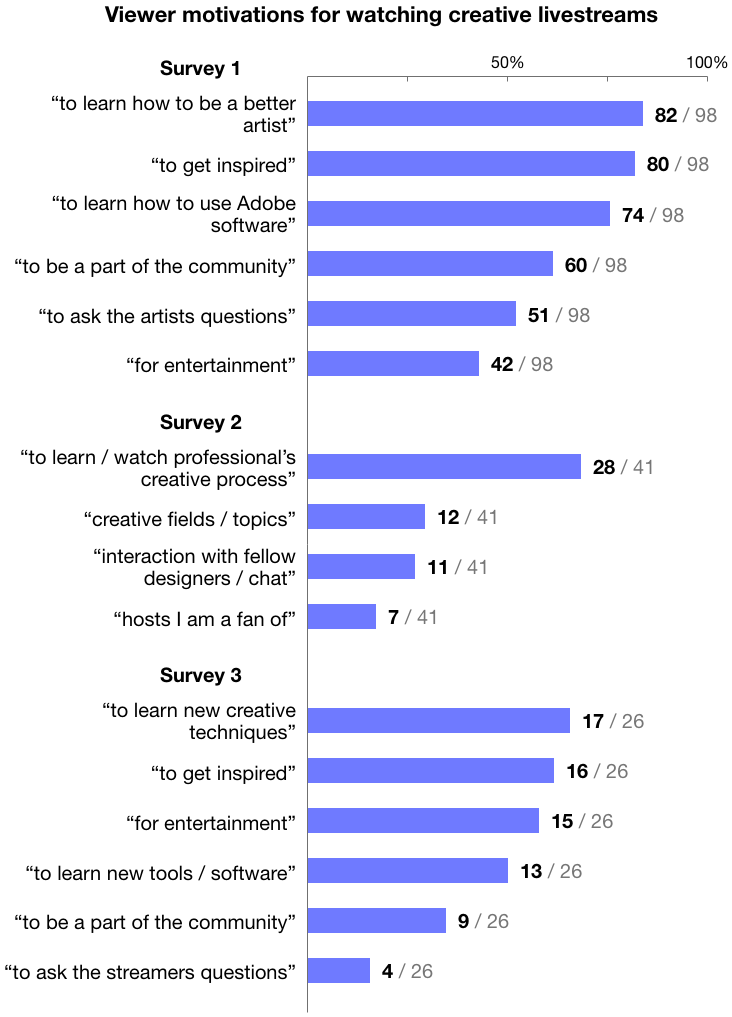
\includegraphics[width=1\columnwidth]{livestreams/figures/survey_responses.png}
  \caption{All three surveys asked why people watch creative livestreams, allowing them to select all answers that applied from a list. This figure shows all responses chosen by at least 15\% of respondents in each survey. }~\label{fig:livestream_survey_responses}
\vspace{-0.15in}
\end{figure}

Almost all free-form elaborations on viewer motivation mentioned learning. Unlike tutorials and lecture videos, livestreams offer direct interaction with the streamer and other viewers, improving the learning experience \cite{Lu2019, Faas2018}. In this way they go beyond just learning content and catalyze ``mentorship communities'' of people with similar interests \cite{Faas2018}. Learners can follow along like an apprentice in a studio, asking questions in the moment. This ability to see authentic, worked examples from start to finish reveals how the streamer makes decisions and recovers from errors \cite{Faas2018}. Viewers often use the knowledge and techniques they learn from creative livestreams to inform their own work, as many \textit{S1} respondents stated in free-form responses. \textit{S3} asked for specific examples; 50\% of respondents provided one. They include adopting new techniques such as photo editing operations, trying out a streamer's creative style for things like musical playing or code commenting, and learning how to achieve a specific goal like fixing a hole in a sweater.


In addition to learning, many also reported watching for inspiration / motivation. With one exception \cite{Cheung2011}, primary work has not reported inspiration as a goal. Cheung \& Huang \cite{Cheung2011} describe ``the Inspired'' as one of nine personas for gaming livestream viewers; watching someone stream the game inspires them to play it themselves. However, a large majority of gaming stream viewers watch for entertainment, learning, or providing commentary. While inspiration can be beneficial in many genres, we believe it is especially salient in creative livestreams due to inspiration's value for creative work \cite{Herring2009}.

In both \textit{S1} and \textit{S3}, inspiration was the second most popular motivation for watching creative livestreams. In addition, 27\% (26/98) of \textit{S1} respondents specifically mentioned inspiration or motivation in free-form responses. 10\% (10/98) also mentioned that the videos helped increase their own motivation and confidence as artists. As one respondent explained, \textit{``[I] like watching artists work because it takes the mystery out of what they do.''} Another said, \textit{``Watching experts make mistakes gives me confidence.''}

Creative work is often a solo activity, and its nebulous nature can make it hard to stay motivated as an artist, often causing creative ``blocks'' such as writer's block. Watching someone else work can motivate viewers to keep going, as well as give them new ideas to try. Respondents in all three surveys mentioned this in free-form responses. For example, one \textit{S1} respondent said they watch livestreams for \textit{``getting myself inspired and hyped before I start working.''} An \textit{S3} participant said, \textit{``It's fun seeing someone else's creative process, and usually motivates me to do my own side projects.''}



%In \textit{S2}, 85\% of respondents said they had watched livestreams of a creative activity they would not have otherwise been interested in, indicating that livestreams can be a good way to discover new topics.

%not directly trying to learn but more get general creative ideas, motivate them to try their own creative projects, and inspire them to see that anyone can do creative things. 


\subsection{Viewers also watch for community and entertainment}
People watch all kinds of livestreams for entertainment \cite{Wohn2018, Lu2018a, Hilvert-Bruce2018, Faas2018, Cheung2011}. It may be the streamer's personality or style, the chat, or the content itself. %Even though livestreams may have long periods of down time with little activity, their unpredictable nature makes them ``engaging but dull'' \cite{Haimson2017}.
People also watch livestreams for community. Viewers often feel emotionally attached to the streamer \cite{Wohn2018, Hu2017}, enjoy connecting and conversing with other viewers \cite{Lu2019, Lu2018, Hilvert-Bruce2018}, and enjoy being able to influence the streamer's content or process in real time \cite{Lu2018a}. Livestream communities often lead to longer-term chat groups on other platforms \cite{Lu2018a, Faas2018}.

All three surveys found community and entertainment to be secondary motivations (\autoref{fig:livestream_survey_responses}), showing that these are also important motivators for creative livestream viewers. Several \textit{S1} respondents valued the company of other creative people while they worked alone. To investigate this further, Surveys 2 and 3 asked what people do while watching livestreams (multiple choice). 68\% (28/41) of \textit{S2} respondents said they watch while doing creative work. 69\% (18/26) of \textit{S3} respondents said they watch while working on something, and 31\% (8/26) said they work on a similar task as the streamer. In this way, creative livestream communities offer a virtual co-working space for people who would otherwise be working alone.

Respondents in all surveys specifically mentioned that the \textit{combination} of learning and entertainment was what drew them to livestreams. This echoes Lu \textit{et al.}'s findings with knowledge-sharing streams \cite{Lu2018a}: they are appealing because they disseminate knowledge in a more relaxed, casual way than tutorials or lecture videos.


%Finally, people watch livestreams for community and social engagement. Viewers of a particular stream share a common interest, and the live chat feature of livestream platforms makes it easy for these viewers to connect with each other as well as with the streamer \cite{Hu2017}. 


\subsection{What are the challenges for viewers?}
\textit{S1} and \textit{S2} asked how the viewing experience might be improved. The most popular suggestions had to do with interactivity and engagement between the streamers and the chat. 17\% (7/41) of \textit{S2} respondents said their questions often get lost in the chat. Busy chat feeds are a problem in other types of livestreams as well \cite{Miller2017}, but can be especially frustrating for viewers seeking to learn and ask questions. Two respondents in \textit{S1} wished that hosts would interact more with the chat, and three others emphasized hosting skill, saying that the best hosts are able to keep the conversation interesting and interact meaningfully with the audience. Two respondents in \textit{S2} wished there were more ways to involve the chat, \textit{e.g.,} through quizzes or polls. Finally, several respondents mentioned that the experience watching replays could be improved; one \textit{S1} respondent said a summary document with important links and tips could help with reviewing the stream later, and three \textit{S2} respondents wished they could view the chat and somehow be involved in the stream when watching replays. This agrees with Lu \textit{et al.}'s findings \cite{Lu2018} that it can be hard to learn from a stream after the fact, as navigation options are usually limited.